\externaldocument{chapter4}
\chapter{Dirt Spot Sweeping Random Strategy}
\label{chap:DSSR}


%%%%%%%%%%%%%%%%%    INTRODUCTION   %%%%%%%%%%%%%%%%%%%%


\section{Introduction}\label{sec:intro4}
The success of a software testing technique is mainly based on the number of faults it discovers in the SUT. An efficient testing process discovers the maximum number of faults in a minimum possible time. Exhaustive testing, where software is tested against all possible inputs, is mostly not feasible because of the large size of input domain, limited resources and strict time constraints. Therefore, strategies in automated software testing tools are developed with the aim to select more failure-finding test inputs from the input domain. Producing such targeted test input is difficult because each system has its own requirements and functionality.

Chan et al.~\cite{chan1996proportional} discovered that there are domains of failure-causing inputs across the input domain. They divided these into point, block and strip domains on the basis of their occurrence across the input domain. Chen et al.~\cite{chen2005adaptive} found that the performance of random testing can be increased by slightly altering the technique of test case selection. In adaptive random testing, they found that the performance increases up to 50\% when test inputs are selected evenly across the whole input domain. This was mainly attributed to the better distribution of input which increased the chance of selecting inputs from failure domains. Similarly Restricted Random Testing \cite{chan2003normalized}, Feedback-Directed Random Testing \cite{pacheco2007randoop}, Mirror Adaptive Random Testing \cite{chen2004mirror} and Quasi Random Testing \cite{chen2007quasi} stress the need for test case selection covering the whole input domain to get better results.

In this chapter we assume that failure domains are contiguous for a significant number of classes. Based on this assumption, we devised the Dirt Spot Sweeping %\footnote{The name refers to the cleaning robots strategy which insists on places where dirt has been found in large amount.} 
Random (DSSR) strategy  which starts as a random+ (R+) strategy focusing more on boundary values. When a new failure is found, it increases the chances of finding more failures by DSSR strategy using the neighbouring values. Since this strategy is an extension of random (R) strategy, it has the full potential to find all failures in the program, but additionally we expect it to be faster at finding failures, for classes in which failure domains are contiguous, as compared with R and R+ strategies.

% to be shifted to result section.


We implemented the DSSR strategy in York Extensible Testing Infrastructure (YETI) \url{http://www.yetitest.org}. To evaluate our approach, we tested 30 times each one of the 60 classes of 32 different projects from the Qualitas Corpus \url{http://www.qualitascorpus.com} with each of the three strategies R, R+ and DSSR. We observed that for 53\% of the classes all three strategies perform equally, for remaining 47\% classes, DSSR strategy performed up to 33\% better than R and up to 17\% better than R+ strategy.

We also validated the approach by comparing the significance of these results using t test and found out that for 7 classes DSSR was significantly better than both R+ and R, for 8 classes DSSR performed similarly to R+ and significantly better than R, while in 2 cases DSSR performed similarly to R and significantly better than R+. In all other classes, DSSR, R+ and R showed no significant difference statistically. Numerically however, the DSSR strategy found 43 more unique failures than R and 12 more unique failures than R+ strategy. 

%The rest of this paper is organised as follows: \\ Section~\ref{sec:dssr} describes the DSSR strategy. Section~\ref{sec:imp} presents implementation of the DSSR strategy. Section~\ref{sec:eval} explains the experimental setup. Section~\ref{sec:res} shows results of the experiments. Section~\ref{sec:discussion3} discusses the results. Section~\ref{sec:rw} presents related work and Section~\ref{sec:conc}, concludes the study.




%%%%%%%%%%%%%%%%%    DIRT SPOT SWEEPING STRATEGY  %%%%%%%%%%%%%%%

\section{Dirt Spot Sweeping Random Strategy}\label{sec:dssr}
The new software testing technique named, Dirt Spot Sweeping Random (DSSR) strategy combines the R+ strategy with a dirt spot sweeping functionality. It is based on two intuitions. First, boundaries have interesting values and using these values in isolation can provide high impact on test results. Second, failures reside more frequently in contiguous blocks and strip domain. If this is true, the Dirt Spot Sweeping (DSS) feature of the strategy will increase the performance of the test. Before presenting the details of the DSSR strategy, it is pertinent to review briefly the R and the R+ strategy.

\subsection{Random Strategy}
The random strategy is a black-box technique in which the SUT is executed using randomly selected test data. Test results obtained are compared to the defined oracle, using SUT specifications in the form of contracts or assertions. In the absence of contracts and assertions the exceptions defined by the programming language are used as test oracles. Because of its black-box nature, this strategy is particularly effective in testing software where the developers want to keep the source code secret~\cite{chen2010adaptive}. The generation of random test data is comparatively cheap and does not require too much intellectual and computational efforts~\cite{ciupa2008finding, ciupa2011number}. It is mainly for this reason that various researchers have recommended R strategy for automated testing tools \cite{ciupa2008artoo}.
 YETI \cite{oriol2010yeti}, AutoTest \cite{leitner2007reconciling, ciupa2007experimental}, QuickCheck \cite{claessen2011quickcheck}, Randoop \cite{pacheco2007feedback} and Jartege \cite{oriat2005jartege} are some of the most common automated testing tools based on R strategy.

\indent Efficiency of random testing was made suspicious with the intuitive statement of Myers \cite{myers2011art} who termed random testing as one of the poorest methods for software testing. However, experiments performed by various researchers, \cite{ciupa2007experimental, hamlet1994random, duran1981report, duran1984evaluation, ntafos2001comparisons} have proved experimentally that random testing is simple to implement, cost effective, efficient and free from human bias as compared to its rival techniques.

Programs tested at random typically fail a large number of times (there are a large number of calls), therefore, it is necessary to cluster failures that likely represent the same fault. The traditional way of doing it is to compare the full stack traces and error types and use this as an equivalence class~\cite{ciupa2007experimental, oriol2012random} called a unique failure. This way of grouping failures is also used for R+ and DSSR.

\subsection{Random+ Strategy}
The random+ strategy~\cite{leitner2007reconciling} is an extension of the R strategy. It uses some special pre-defined values which can be boundary values or values that have high tendency of finding failures in the SUT. Boundary values~\cite{beizer2003software} are the values on the start and end of a particular type. For instance, such values for \verb+int+ could be \verb+MAX_INT+, \verb+MAX_INT-1+, \verb+MAX_INT-2+; \verb+MIN_INT+, \verb-MIN_INT+1-, \verb-MIN_INT+2-. These special values can add a significant improvement to any testing method. For example:

\begin{lstlisting}
public void test (int arg) {
	arg = arg + 1;
	int [] intArray = new intArray[arg];
	...
}
\end{lstlisting}

In the above piece of code, on passing interesting value \verb+MAX_INT+ as argument, the code increment it by 1 making it a negative value and thus an error is generated when the system tries to build an array of negative size. 

Similarly, the tester might also add some other special values that he considers effective in finding failures for the SUT. For example, if a program under test has a loop from -50 to 50 then the tester can add -55 to -45, -5 to 5 and 45 to 55 to the pre-defined list of special values. This static list of interesting values is manually updated before the start of the test and has high priority than selection of random values because of more relevance and high chances of finding failures for the given SUT. These special values have high impact on the results, particularly for detecting problems in specifications~\cite{ciupa2008finding}.


\subsection{Dirt Spot Sweeping}
Chan et al.~\cite{chan1996proportional} found that there are domains of failure-causing inputs across the input domain. Section~\ref{sec:failuredomains_2} shows these domains for two-dimensional input domain. They divided these domains into three types called point, block and strip domains. The black area inside the box in the form of points, block and strip shows the input which causes the system to fail while white area inside the box represent the genuine input. Boundary of the box (black solid line) surrounds the complete input domain and represents the boundary values. They argue that a strategy has more chances of hitting these failure domains if test cases far away from each other are selected. Other researchers~\cite{chen2004mirror, chan2003normalized, chen2007quasi}, also tried to generate test cases further away from one another targeting these domains and achieved better performance. The increase in performance indicates that failures more often occur contiguously across the input domain. When test value reveals a failure in a program then DSS may not look farthest away for the selection of next test value but picks the closest test values for the next several tests to find another failure from the same region.

%\begin{figure} [H]
%\centering
%\subfigure[Point domain]{
%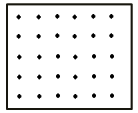
\includegraphics[width=3.6cm,height=3.6cm]{chapter4/point.png}
%\label{fig:point}
%}
%\subfigure[Block domain]{
%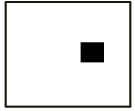
\includegraphics[width=3.6cm,height=3.6cm]{chapter4/block.png}
%\label{fig:block}
%}
%\subfigure[Strip domain]{
%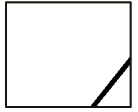
\includegraphics[width=3.6cm,height=3.6cm]{chapter4/strip.png}
%\label{fig:strip}
%}

%\caption{Failure domains across input domain~\cite{chan1996proportional}}
%\label{fig:patterns3}
%\end{figure}



%\begin{figure}[ht]                                    
%\centering
%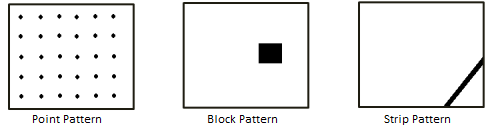
\includegraphics[width= 10cm,height=4cm]{chapter4/ART_Patterns.png}
%\caption{Failure domains across input domain~\cite{chan1996proportional}}
%\label{fig:patterns3}
%\end{figure}

Dirt spot sweeping is the feature of DSSR strategy that comes into action when a failure is found in the system. On finding a failure, it immediately adds the value causing the failure and its neighbouring values to the existing list of interesting values. For example, in a program when the \verb+int+ type value of 50 causes a failure in the system then spot sweeping will add values from 47 to 53 to the list of interesting values. If the failure lies in the block or strip domain, then adding it's neighbouring values will explore other failures present in the block or strip. In DSSR strategy the list of interesting values is dynamic and changes during the test execution of each program. While in R+ strategy, the list of interesting values remain static and manually changed before the start of each test.

\begin{figure}[ht]
\centering
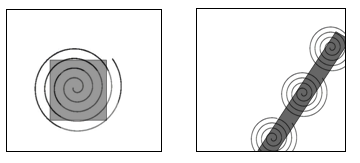
\includegraphics[width=10cm,height=4cm]{chapter4/block2.png}
\caption{Exploration of failures by DSS in block and strip domain}
\label{fig:block2}
\end{figure}

Figure \ref{fig:block2} shows how DSS explores the failures residing in the block and strip domains of a program. The coverage of block and strip domain is shown in spiral form because first failure leads to second, second to third and so on till the end. In case the failure is positioned on the point domain then the added values may not be effective because point domain is only an arbitrary failure point in the whole input domain.

\subsection{Working of DSSR Strategy}

The DSSR strategy continuously tracks the number of failures during the execution of the test. This tracking is done in a very effective way with zero or minimum overhead~\cite{leitner2009effectiveness}. The test execution is started by R+ strategy and continues till a failure is found in the SUT after which the program copies the values leading to the failure as well as the surrounding values to the dynamic list of interesting values. 

\begin{figure}[ht]
\centering
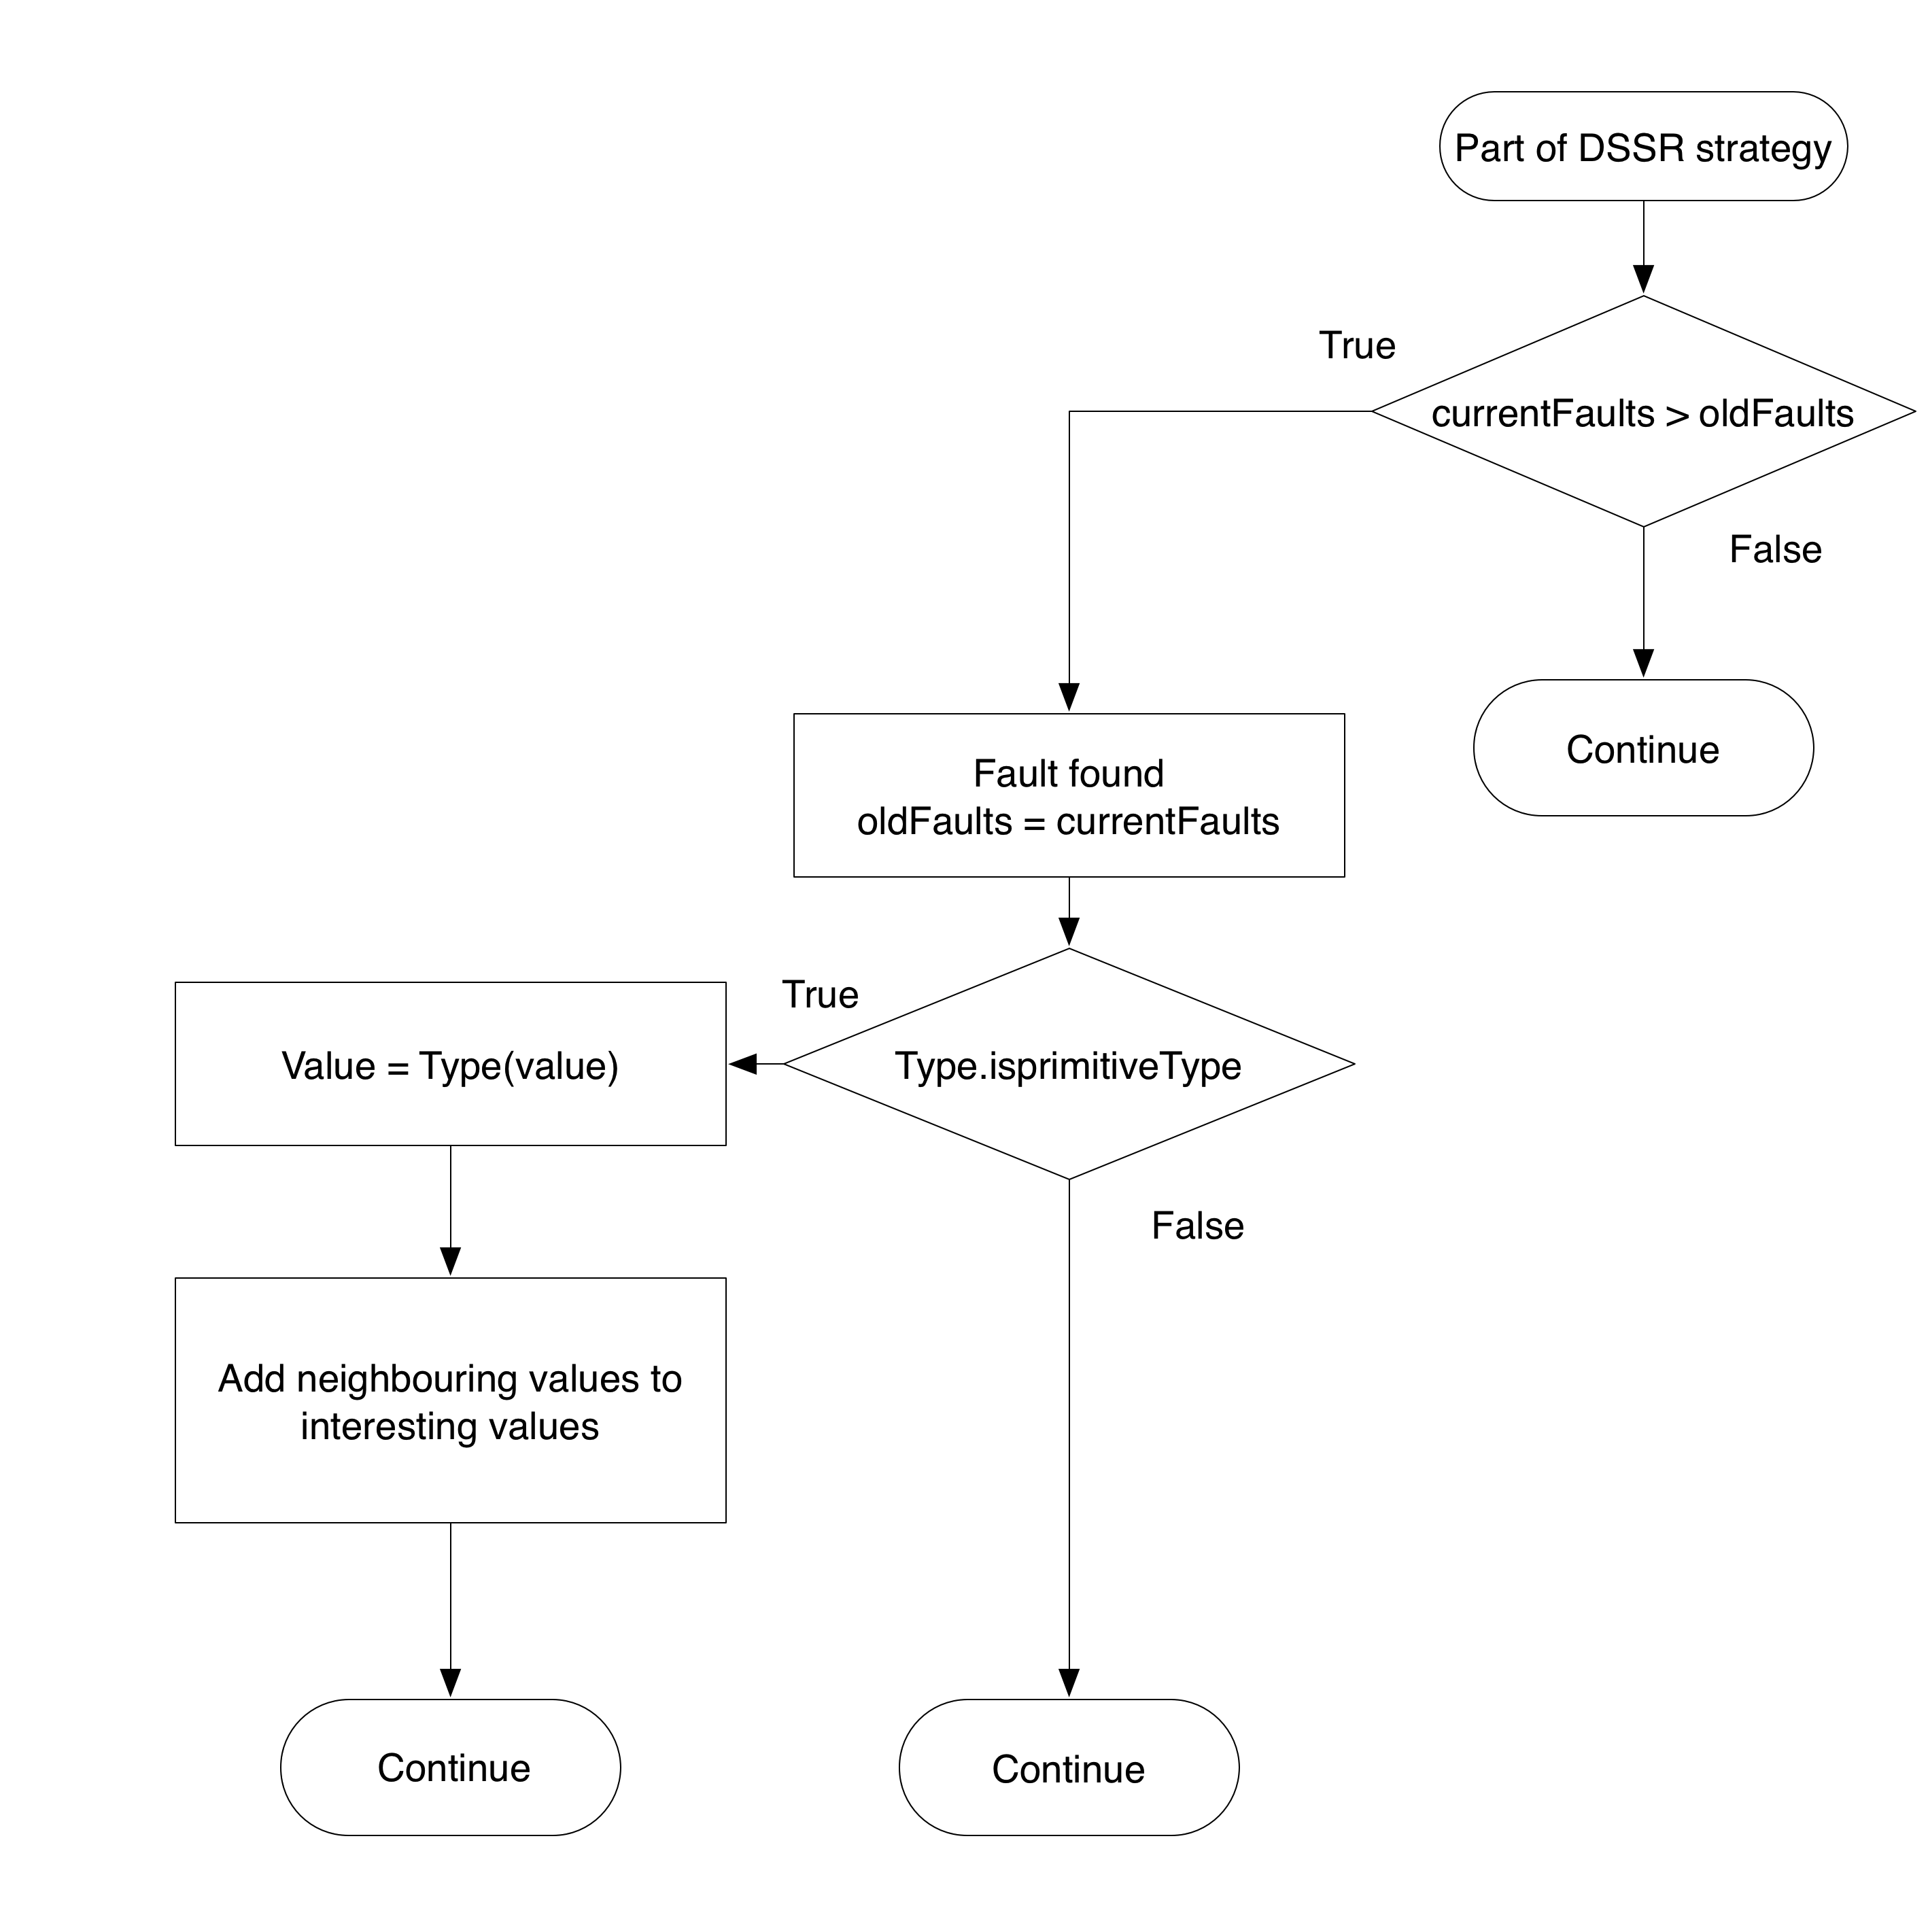
\includegraphics[width=12cm, height=14cm]{chapter4/flowchart1.png}
\caption{Working mechanism of DSSR Strategy}
\label{fig:Working_DSSS}
\end{figure}

The flowchart presented in Figure~\ref{fig:Working_DSSS} depicts that, when the failure finding value is of primitive type, the DSSR strategy identifies its type and add values only of that particular type to the list of interesting values. The resultant list of interesting values provides relevant test data for the remaining test session and the generated test cases are more targeted towards finding new failures around the existing failures in the given SUT.

Boundary and other special values having a high tendency of finding failures in the SUT are added to the list of interesting values by R+ strategy prior to the start of test session where as in DSSR strategy the failure-finding and its surrounding values are added at runtime when a failure is found. 

Table \ref{table:addvalues2} presents the values added to the list of interesting values when a failure is found. In the table the test value is represented by $X$ where $X$ can be a primitive type, string or user defined objects. All values are converted to their respective types before adding them to the list of interesting values.



%%%%%%%%%%%%%%%%%%%%%%%%%%%%%%%%%%%%



\begin{table}[ht]
%\scriptsize
\caption{Data types and Corresponding values to be added} % title of Table
\centering % used for centering table
{\renewcommand{\arraystretch}{1.5} 
\begin{tabular}{| l | l |} % centered columns (4 columns)
\hline\hline %inserts double horizontal lines
Data Type & Values to be added\\ [0.5ex] % inserts table
%heading
\hline % inserts single horizontal line
\multirow{1}{*}{X is int, double, float, } & X,  X+1, X+2, X+3,  \\ % inserting body of the
\multirow{1}{*}{long, byte, short \& char} & X-1, X-2, X-3 \\ 

\hline
\multirow{8}{*}{X is String} & X\\ % inserting body of the table

& X + ``  "\\ % inserting body of the table
& ``  " + X \\ % inserting body of the table
& X.toUpperCase() \\
& X.toLowerCase() \\
& X.trim() \\
& X.substring(2) \\
& X.substring(1, X.length()-1) \\
\hline
\multirow{1}{*}{X is object of user} & Call its constructor recursively \\ % inserting body of the
\multirow{1}{*}{defined class} & until empty or primitive values \\[1ex]
\hline
\hline %inserts single line
\end{tabular}
}
\bigskip
\label{table:addvalues2} % is used to refer this table in the text
\end{table}



%%%%%%%%%%%%%%%%%%%%%%%%%%%%% EXPLANATION OF DSSR STRATEGY %%%%%%%%%%%%%%%%%%%%%%%%%%


\subsection{Explanation of DSSR Strategy by Example}
The DSSR strategy is explained through a simple program seeded with three fault. The first fault is a division by zero exception denoted by 1 while the second and third faults are failing assertion denoted by 2 and 3 in the given program below: 

\begin{lstlisting}
/** 
* Calculate square of given number 
* and verify results. 
* The code contain 3 faults.
* @author (Mian and Manuel)
*/
public class Math1 {
 public void calc (int num1) {
  // Square num1 and store result. 
  int result1 = num1 * num1;
  int result2 = result1 / num1; // (1)
  assert Math.sqrt(result1) == num1; // (2)
  assert result1 >= num1; // (3)
 } 
}
\end{lstlisting}

In the above code, one primitive variable of type \verb+int+ is used, therefore, the input domain for DSSR strategy is from \verb+-2,147,483,648 to 2,147,483,647+. The strategy further select values (\verb+0, Integer.MIN_VALUE+ \& \verb+Integer.MAX_VALUE+) as interesting values which are prioritised for selection as inputs. 
As the test starts, three failures are quickly discovered by DSSR strategy in the following order.

\indent \textbf{Failure 1:} The strategy select value \verb+0+ for variable \verb+num1+  in the first test case because \verb+0+ is available in the list of interesting values and therefore its priority is higher than other values. This will cause violation of assertion (1) and Java to generate division by zero exception.

\indent \textbf{Failure 2:} After discovering the first failure, the strategy adds it and its surrounding values to the list of interesting values i.e. \verb+0, 1, 2, 3 and -1, -2, -3+ in this case. In the second test case the strategy may pick \verb+-3+ as a test value which may lead to the second failure where assertion (2) fails because the square root of \verb+9+ is \verb+3+ instead of the input value -3.

\indent \textbf{Failure 3:} After a few tests the strategy may select \verb+Integer.MAX_VALUE+ for variable \verb+num1+  from the list of interesting values leading to the discovery of 3rd failure because int variable \verb+result1+ will not be able to store the square of \verb+Integer.MAX_VALUE+. Instead of the actual square value Java assigns a negative value (Java language rule) to variable \verb+result1+ that will lead to the violation of the next assertion (3).

The above process explains that including the border, failure-finding and surrounding values to the list of interesting values in DSSR strategy leads to the available failures quickly and in fewer tests as compared to R and R+ strategy. R and R+ takes more number of tests and time to discover the second and third failures because in these strategies the search for new unique failures starts again randomly in spite of the fact that the remaining failures lie in close proximity to the first one.




\begin{figure}[H]
\centering
\setlength{\fboxsep}{0pt}%
\setlength{\fboxrule}{1pt}%
\fbox{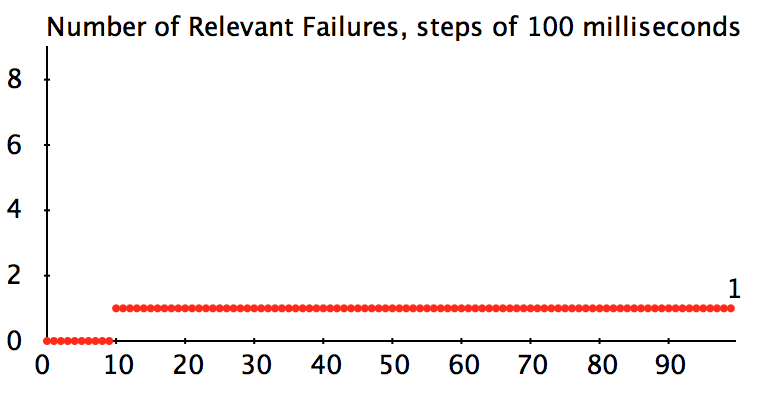
\includegraphics[width=15cm,height=9cm]{chapter4/random.png}}
\caption{Test result of random strategy for the example code}
\label{fig:random_result}
\end{figure}

\bigskip

\begin{figure}[H]
\centering
\setlength{\fboxsep}{0pt}%
\setlength{\fboxrule}{1pt}%
\fbox{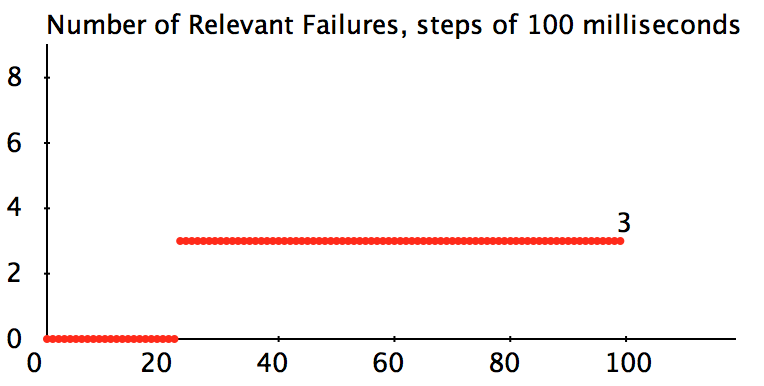
\includegraphics[width=15cm,height=9cm]{chapter4/DSSR.png}}
\caption{Test result of DSSR strategy for the example code}
\label{fig:dssr_result}
\end{figure}


%%%%%%%%%%%%%%%%%    IMPLEMENTATION OF DSSR STRATEGY   %%%%%%%%%%%%


\section{Implementation of DSSR Strategy}\label{sec:imp}

The DSSR strategy is implemented in YETI open-source automated random testing tool. YETI, coded in Java language, is capable of testing systems developed in procedural, functional and object-oriented languages. Its language-agnostic meta model enables it to test programs written in multiple languages including Java, C\#, JML and .Net. The core features of YETI include easy extensibility for future growth, high speed (up to one million calls per minute on java code), real time logging, real time GUI support, capability to test programs with multiple strategies and auto generation of test report at the end of test session. For large-scale testing there is a cloud-enabled version of YETI, capable of executing parallel test sessions in the cloud~\cite{oriol2010yeti}. A number of hitherto failures have successfully been found by YETI in various production software~\cite{oriol2012random}.

YETI can be divided into three decoupled main parts: the core infrastructure, language-specific bindings and strategies. The core infrastructure contains representation for routines, a group of types and a pool of specific type objects. The language specific bindings contain the code to make the call and process the results. The strategies define the procedure of selecting the modules (classes), the routines (methods) and generation of values for instances involved in the routines. By default, YETI uses R strategy if no particular strategy is defined during test initialisation. It also enables the user to control the probability of using null values and the percentage of newly created objects for each test session. YETI provides an interactive Graphical User Interface (GUI) in which users can see progress of the current test in real time. In addition to GUI, YETI also provides extensive logs of the test session for more in-depth analysis.

The DSSR strategy is an extension of YetiRandomPlusStrategy. The class hierarchy is shown in Figure \ref{fig:hierarchyofDSSR}.

\begin{figure}[h]
\centering
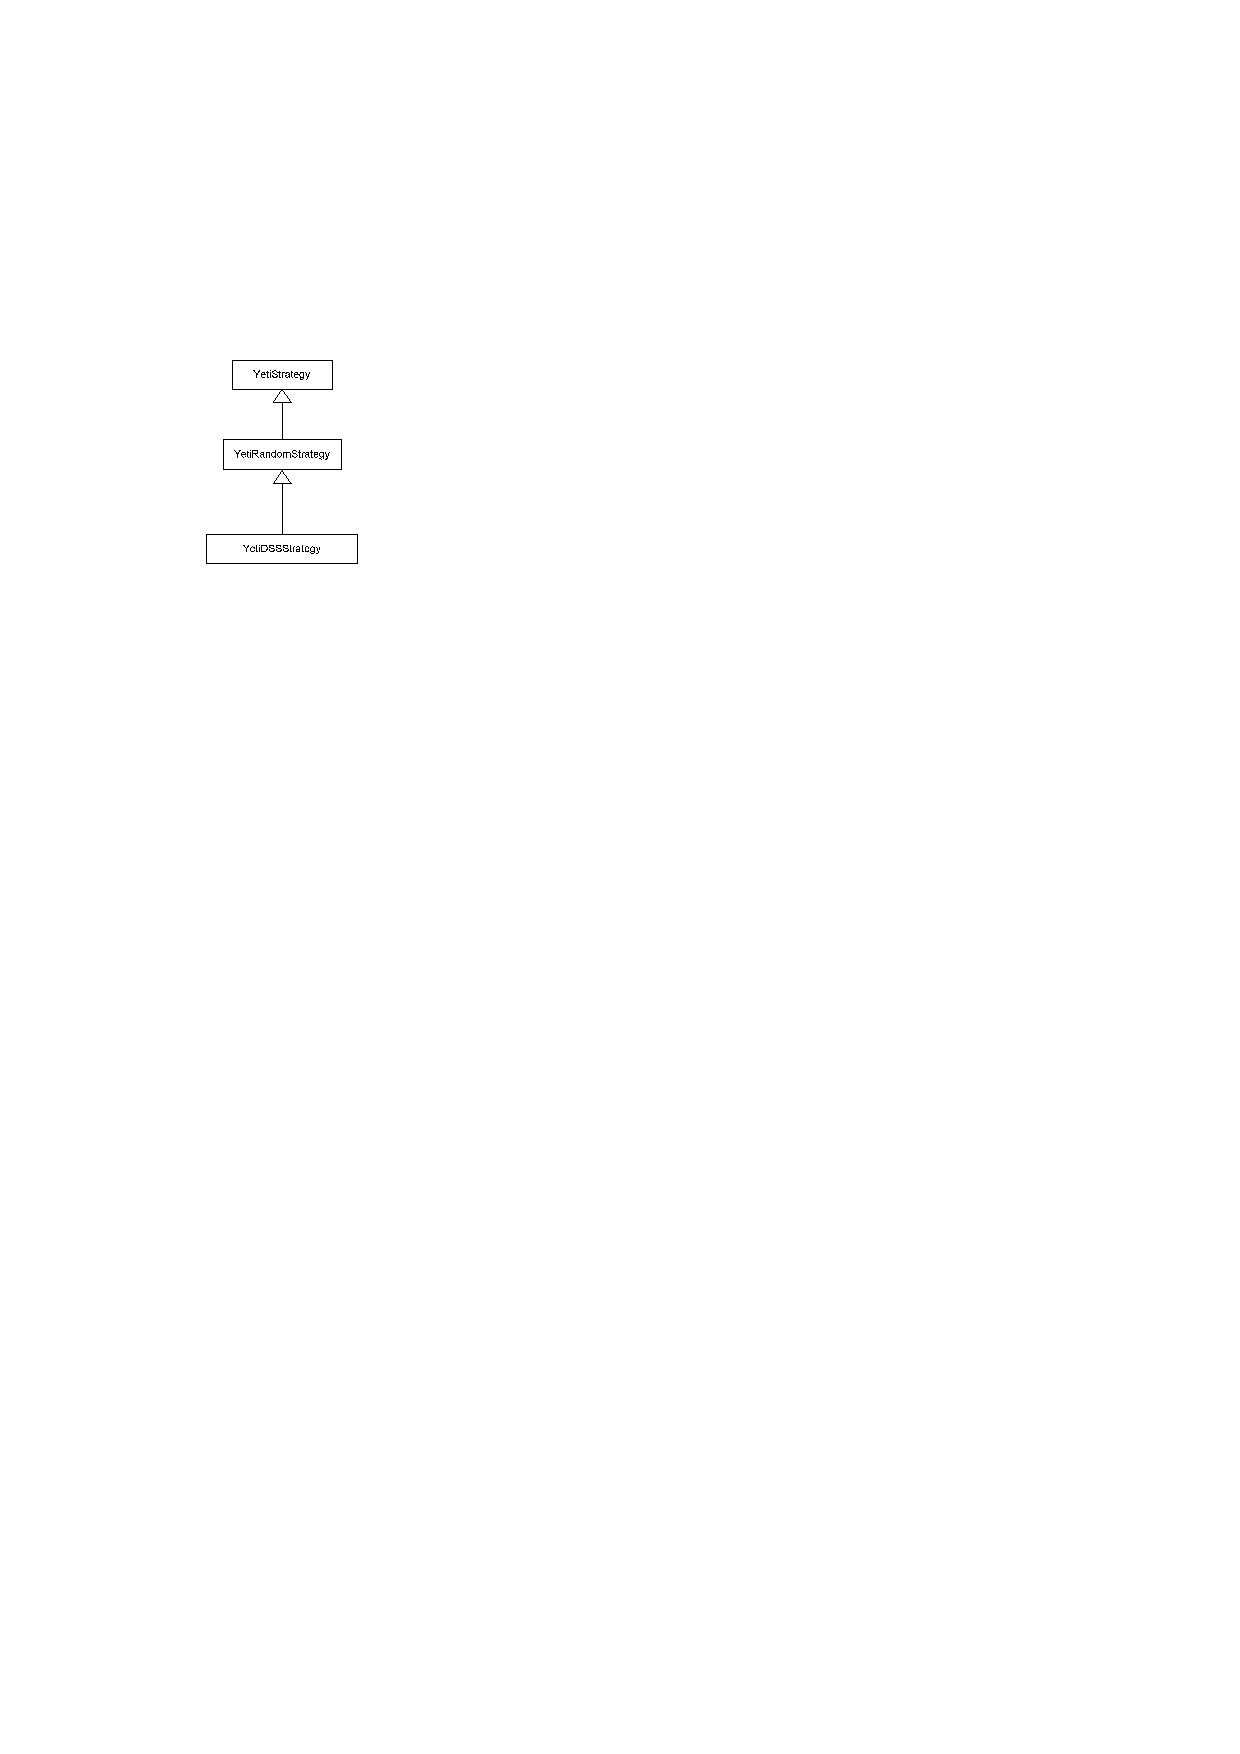
\includegraphics[width=7cm,height=9cm]{chapter4/hierarchy.pdf}
\caption{Class Hierarchy of DSSR in YETI}
\label{fig:hierarchyofDSSR}
\end{figure}





%%%%%%%%%%%%%%%%%    EVALUATION   %%%%%%%%%%%%%%%%%%%%


\section{Evaluation}\label{sec:eval}

The DSSR strategy is experimentally evaluated by comparing its performance with that of R and R+ strategy ~\cite{leitner2007reconciling}. General factors such as system software and hardware, YETI specific factors like percentage of null values, percentage of newly created objects and interesting value injection probability have been kept constant in the experiments.

\subsection{Research Questions}
For evaluating the DSSR strategy, the following research questions have been addressed in this study:
\begin{enumerate}
\item Is there an absolute best amongst R, R+ and DSSR strategies?
\item Are there classes for which any of the three strategies provide better results?
\item Can we pick the best default strategy amongst R, R+ and DSSR?
\end{enumerate}



\subsection{Experiments}
We performed extensive testing of programs from the Qualitas Corpus~\cite{tempero2010empirical}. The Qualitas Corpus is a curated collection of open source Java projects built with the aim of helping empirical research in the field of software engineering. These projects have been collected in an organised form containing the source and binary forms. The Qualitas Corpus [version 20101126] containing 106 open source Java projects was used in the current evaluation. In our experiments we randomly selected 60 classes from 32 projects taken at random. All the selected classes produced at least one failure and did not time out with maximum testing session of 10 minutes. Every class was tested thirty times by each strategy (R, R+, DSSR). Name, version and size of the projects to which the classes belong are given in Table~\ref{table:projects} while test details of the classes are presented in Table~\ref{table:Results}. Line of Code (LOC) tested per class and the total LOC's tested are shown in column 3 of Table~\ref{table:Results}. 

Every class is evaluated through $10^5$ calls in each test session. %\footnote{The total number of tests is thus \verb+60\times 30\times 3 \times 10^5 = 540\times 10^6~tests+.} 
The approach similar to that used in previous studies when the contracts and assertions in the code under test are absent was followed in the study~\cite{oriol2012random}. The undeclared exceptions were treated as failures.


\begin{table}[htp]
\caption{Specifications of projects randomly selected from Qualitas Corpus}
\bigskip
\centering
{\renewcommand{\arraystretch}{1.2} %<- modify value to suit your needs
\begin{tabular}{rlrr}

{\textbf {S. No}}& 	{\textbf {Project Name}}	& 	{\textbf {Version}}		&	{\textbf {Size (MB)}}\\
1	&	apache-ant	&	1.8.1			&	59\\
2	&	antlr		&	3.2				&	13\\
3	&	aoi			&	2.8.1			&	35\\
4	&	argouml		&	0.30.2			&	112\\
5	&	artofillusion	&	281				&	5.4\\
6	&	aspectj		&	1.6.9			&	109.6\\
7	&	axion		&	1.0-M2			&	13.3\\
8	&	azureus		&	1				&	99.3\\
9	&	castor		&	1.3.1			&	63.2\\
10	&	cayenne		&	3.0.1			&	4.1\\
11	&	cobertura	&	1.9.4.1			&	26.5\\
12	&	colt			&	1.2.0			&	40\\
13	&	emma		&	2.0.5312		&	7.4\\
14	&	freecs		&	1.3.20100406	&	11.4\\
15	&	hibernate	&	3.6.0			&	733\\
16	&	hsqldb		&	2.0.0			&	53.9\\
17	&	itext		&	5.0.3			&	16.2\\
18	&	jasml		&	0.10			&	7.5 \\
19	&	jmoney		&	0.4.4			&	5.3\\
20	&	jruby		&	1.5.2			&	140.7\\
21	&	jsXe			&	04\_beta		&	19.9\\
22	&	quartz		&	1.8.3			&	20.4\\
23	&	sandmark	&	3.4				&	18.8\\
24	&	squirrel-sql	&	3.1.2			&	61.5\\
25	&	tapestry		&	5.1.0.5			&	69.2\\
26	&	tomcat		&	7.0.2			&	24.1\\
27	&	trove		&	2.1.0			&	18.2\\
28	&	velocity		&	1.6.4			&	27.1\\
29	&	weka		&	3.7.2			&	107\\
30	&	xalan		&	2.7.1			&	85.4\\
31	&	xerces		&	2.10.0			&	43.4\\
32	&	xmojo		&	5.0.0			&	15\\
%\hline
\end{tabular}
}
\bigskip
\label{table:projects}
\end{table}



All tests are performed with a 64-bit Mac OS X Lion [version 10.7.4] running on 2 x 2.66 GHz 6-Core Intel Xeon processor with 6 GB (1333 MHz DDR3) of RAM. YETI runs on top of the Java\texttrademark  SE Runtime Environment [version 1.6.0\_35]. The machine took approximately 100 hours to process the experiments.


\subsection{Performance Measurement Criteria} \label{measurementCriteria_4}
Various measures including the E-measure (expected number of failures detected), P-measure (probability of detecting at least one failure) and F-measure (number of test cases used to find the first failure) have been reported in the literature for finding the effectiveness of R strategy. The E-measure and P-measure have been criticised~\cite{chen2005adaptive} and are not considered effective measuring techniques while the F-measure has been often used by various researchers~\cite{chen2004statistical, chen1996expected}. In our initial experiments, the F-measure was used to evaluate the efficiency of test strategy. However it was later realised that this was not the right choice. In some experiments a strategy found the first failure quickly than the other but on completion of test session that very strategy found lower number of total failures than the rival strategy. The preference given to a strategy by F-measure because it finds the first failure quickly without giving due consideration to the total number of failures is not fair~\cite{liu2012comparison}.


  
The literature review revealed that the F-measure is used where testing stops after identification of the first failure and the system is given back to the developers to remove the fault. Currently automated testing tools test the whole system and print all discovered failures in one go and F-measure is not the favourable choice. In our experiments, performance of the strategy was measured by the maximum number of failures detected in SUT by a particular number of test calls \cite{ciupa2007experimental, pacheco2007feedback, ciupa2008predictability}. This measurement was effective because it considers the performance of the strategy when all other factors are kept constant.



%%%%%%%%%%%%%%%%%    RESULTS   %%%%%%%%%%%%%%%%%%%%

\begin{figure}[h]
	\centering
	\centerline{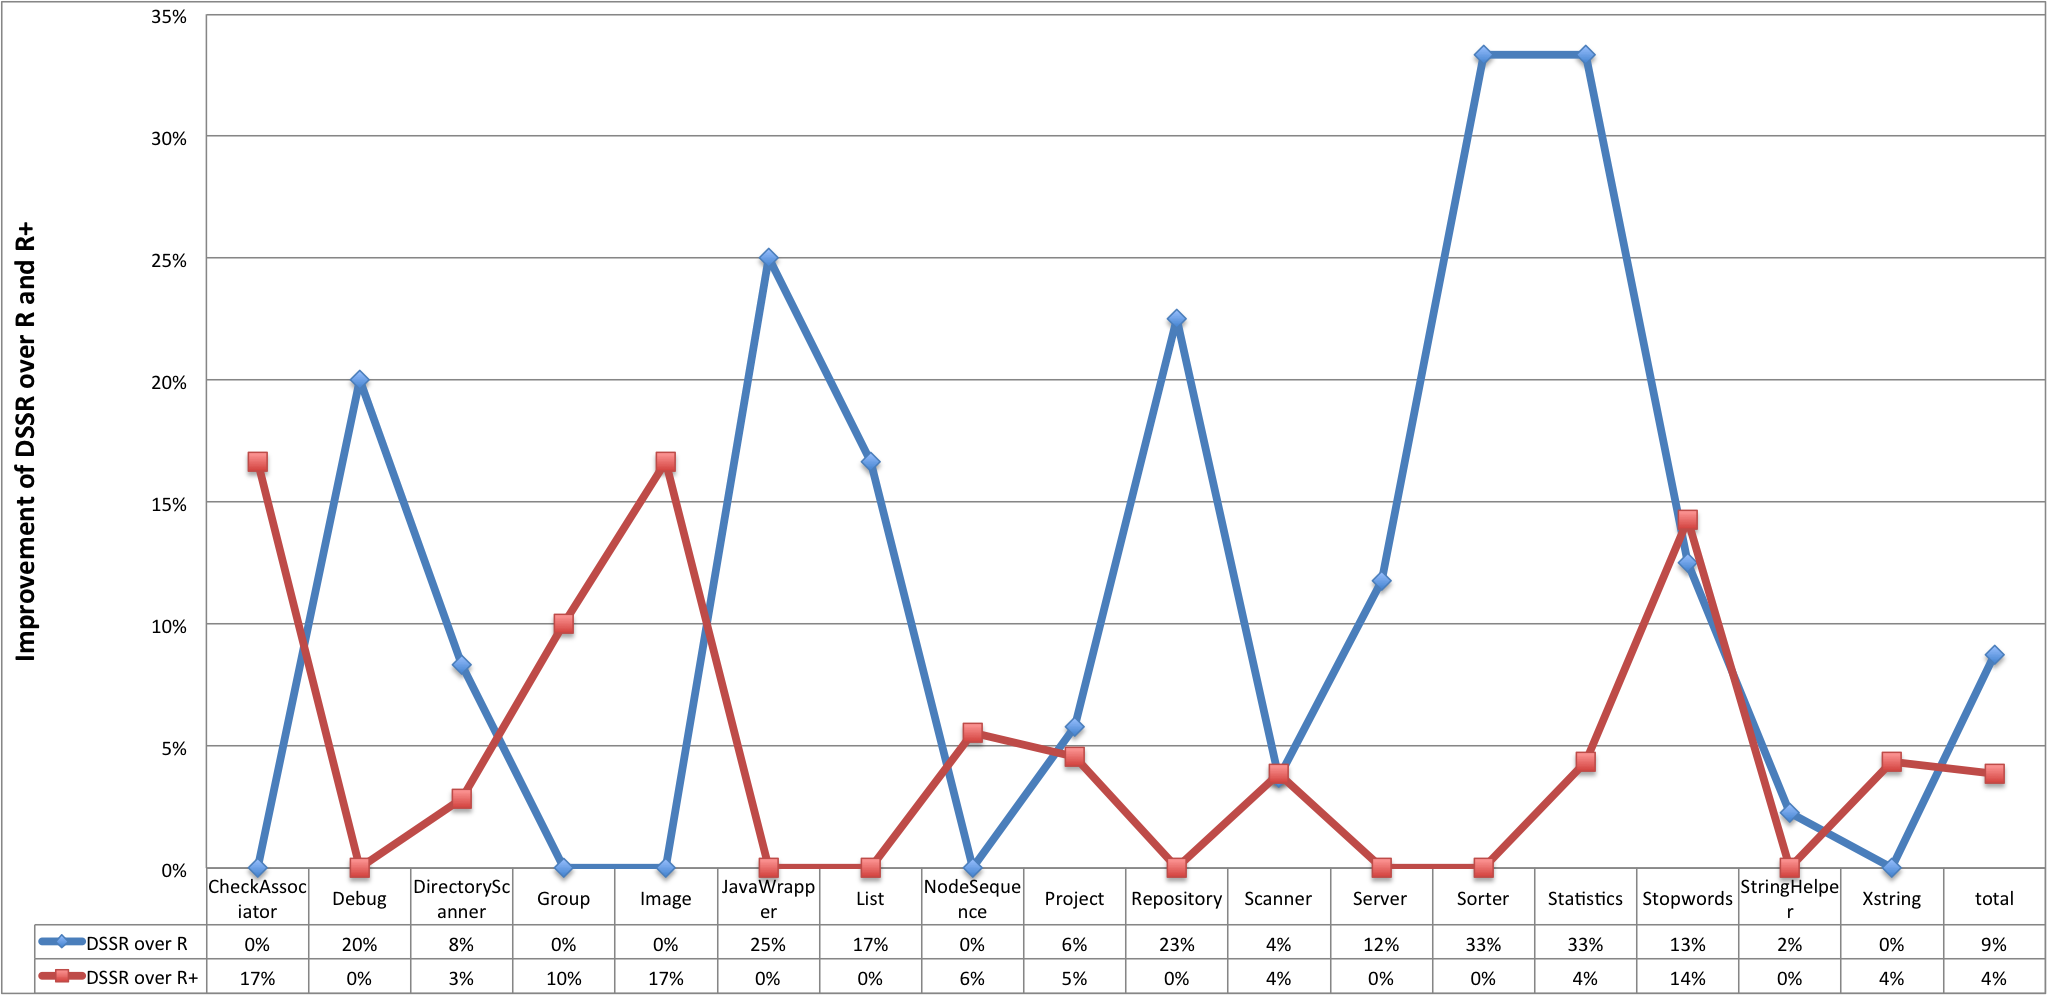
\includegraphics[width=16cm, height=12cm]{chapter4/DssrImprove.png}}
	\caption{Performance of DSSR in comparison with R and R+ strategies.}
	\label{fig:LineChart}
\end{figure}


%\begin{figure}[h]
%\centerline{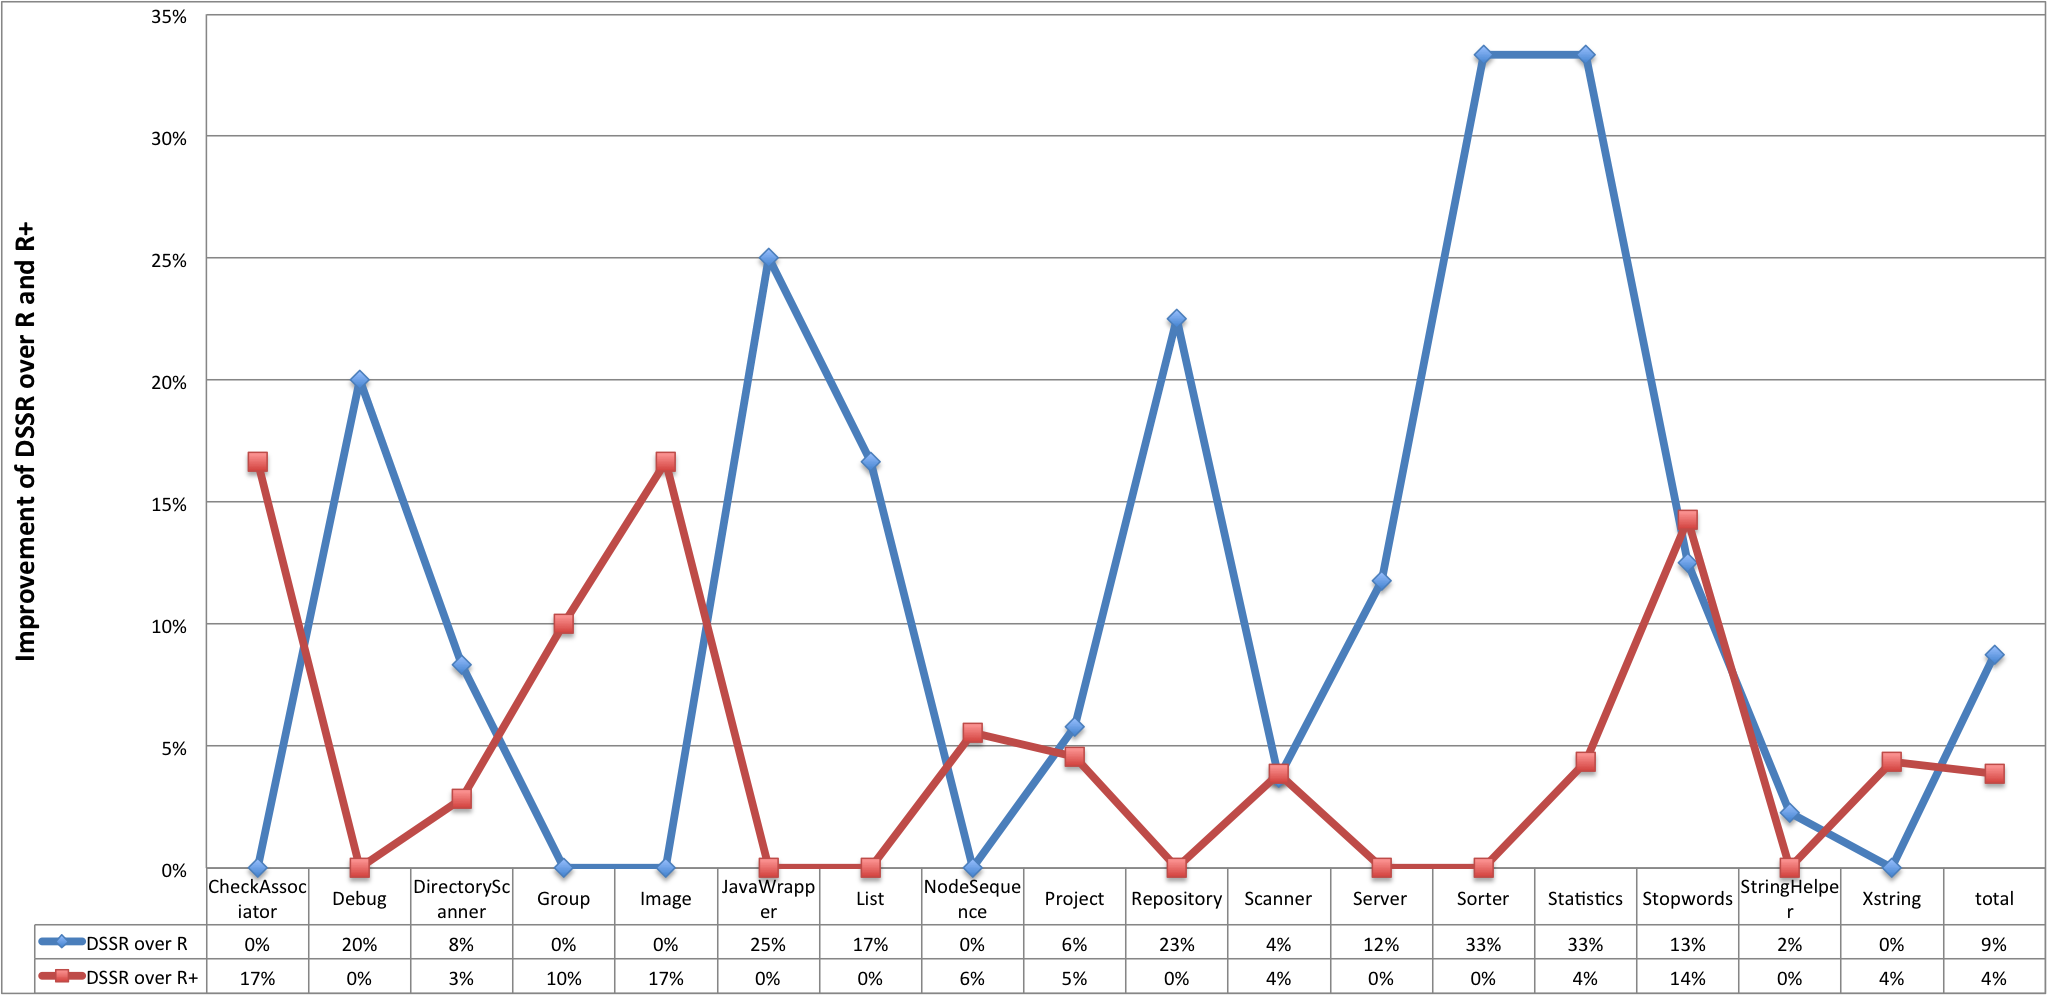
\includegraphics[width=16.5cm,height=9cm]{chapter4/DssrImprove.png}}
%\centerline{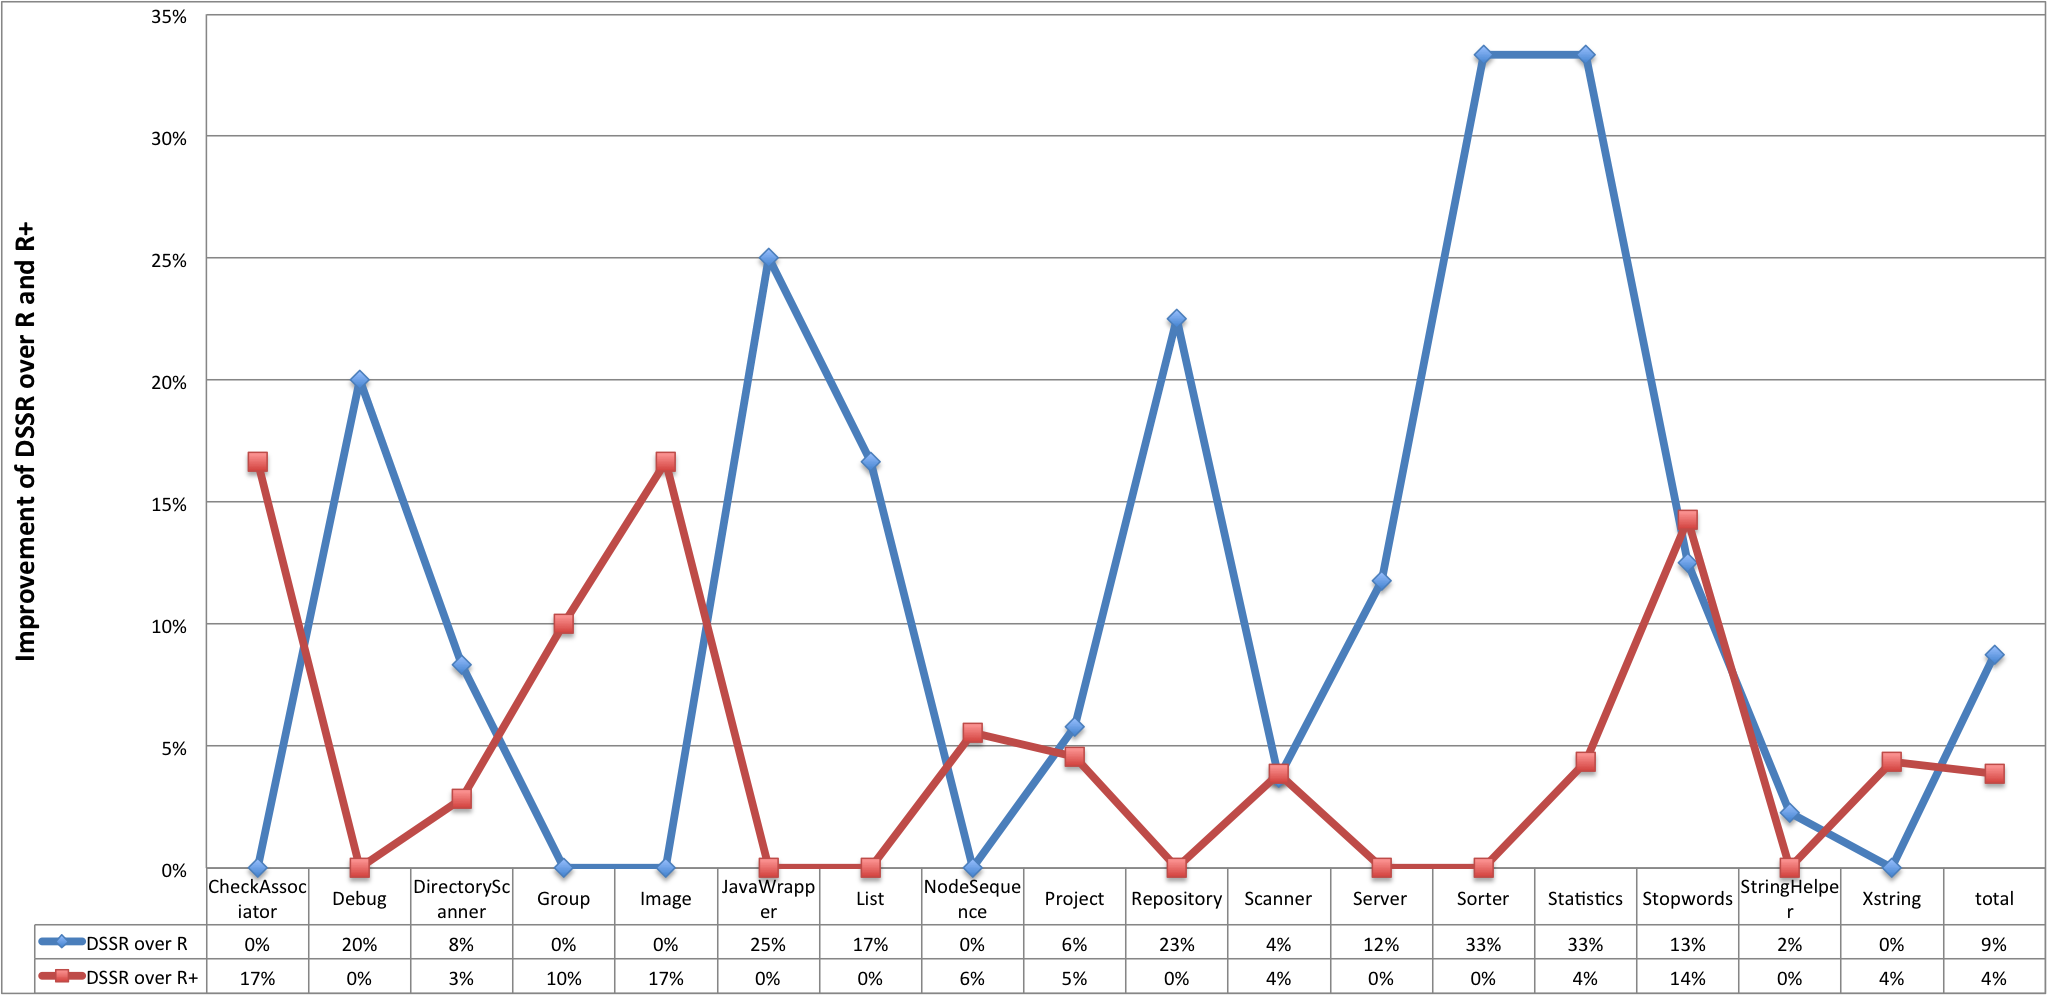
\includegraphics[width=16cm,height=9cm]{chapter4/DssrImprove.png}}
%\caption{Performance of DSSR in comparison with R and R+ strategies.}
%\label{fig:LineChart}
%\end{figure}

%%%%%%%%%%%%%%%%%%%%%%%%%%%%%%%%%%%%%%%%%%%%



\begin{table*} [htp!]
  \scriptsize
 \caption{Comparative performance of R, R+ and DSSR strategies}
	%\begin{minipage}[h]{\pagewidth}\centering
	\bigskip
	\hspace{-2.2cm}
	\noindent\makebox[\textwidth]{
 	\begin{tabularx}{1 \textwidth}{r l r r r r r r r r r r r r r}
      %\aline

      \multirow{2}{*}{{\textbf {S. No}}}		& \multirow{2}{*}{{\textbf {Class Name}}}		& \multirow{2}{*}{{\textbf {LOC}}}	& \multicolumn{4}{c}{{\textbf {R}}}							&	\multicolumn{4}{c}{{\textbf {R+}}}							&	\multicolumn{4}{c}{{\textbf {DSSR}}}	\\
      %\cline{3-14} 
      						&						&			& Mean 	& Max	& Min 	& 	R-STD				& Mean 	& Max 	& Min 	&	 R-STD 			& Mean 		& Max 		& Min		& R-STD \\
      						


1						& ActionTranslator			&709		& 96		&	96	&	96	& 	0					& 96		& 96 		& 96		& 		0			& 96			& 96			& 96			&	0\\     
2						& AjTypeImpl				&1180		& 80		&	83	&	79	& 	0.02					& 80		& 83 		& 79		& 		0.02			& 80			& 83			& 79			&	0.01\\      
\textbf{3}					& \textbf{Apriori}			&\textbf{292}	& \textbf{3}&	\textbf{4}	&\textbf{3}	& \textbf{0.10}			& \textbf{3}& \textbf{4} 		& \textbf{3}& \textbf{0.13}	& \textbf{3}	& \textbf{4}	& \textbf{3}	&\textbf{0.14}\\      
4						& BitSet					&575		& 9		&	9	&	9	& 	0					& 9		& 9 		& 9		& 		0			& 9			& 9			& 9			&	0\\       
5						& CatalogManager			&538		& 7		&	7	&	7	& 	0					& 7		& 7 		& 7		& 		0			& 7			& 7			& 7			&	0\\    
\textbf{6}					& \textbf{CheckAssociator}	&\textbf{351}	& \textbf{7}	&	\textbf{8}	&	\textbf{2}	& 	\textbf{0.16}					& \textbf{6}		& \textbf{9} 		& \textbf{2}		& 		\textbf{0.18}			& \textbf{7}			& \textbf{9}			& \textbf{6}			&	\textbf{0.73}\\    
\textbf{7}						& \textbf{Debug}					&\textbf{836}		& \textbf{4}		&	\textbf{6}	&	\textbf{4}	& 	\textbf{0.13}					& \textbf{5}		& \textbf{6} 		& \textbf{4}		& 		\textbf{0.12}			& \textbf{5}			& \textbf{8}			& \textbf{4}			&	\textbf{0.19}\\       
\textbf{8}						& \textbf{DirectoryScanner}			&\textbf{1714}		& \textbf{33}		&	\textbf{39}	&	\textbf{20}	& 	\textbf{0.10}					& \textbf{35}		& \textbf{38} 		& \textbf{31}		& 		\textbf{0.05}			& \textbf{36}			& \textbf{39}			& \textbf{32}			&	\textbf{0.04}\\      
9						& DiskIO					&220		& 4		&	4	&	4	& 	0					& 4		& 4 		& 4		& 		0			& 4			& 4			& 4			&	0\\      
10						& DOMParser				&92			& 7		&	7	&	3	& 	0.19					& 7		& 7 		& 3		& 		0.11			& 7			& 7			& 7			&	0\\      
11						& Entities					&328		& 3		&	3	&	3	& 	0					& 3		& 3 		& 3		& 		0			& 3			& 3			& 3			&	0\\      
12						& EntryDecoder			&675		& 8		&	9	&	7	& 	0.10					& 8		& 9 		& 7		& 		0.10			& 8			& 9			& 7			&	0.08\\   
13						& EntryComparator			&163		& 13		&	13	&	13	& 	0					& 13		& 13 		& 13		& 		0			& 13			& 13			& 13			&	0\\      
14						& Entry					&37			& 6		&	6	&	6	& 	0					& 6		& 6 		& 6		& 		0			& 6			& 6			& 6			&	0\\   
15						& Facade					&3301		& 3		&	3	&	3	& 	0					& 3		& 3 		& 3		& 		0			& 3			& 3			& 3			&	0\\   
16						& FileUtil					&83			& 1		&	1	&	1	& 	0					& 1		& 1 		& 1		& 		0			& 1			& 1			& 1			&	0\\      
17						& Font					&184		&12		&	12	&	11	& 	0.03					& 12		& 12 		& 11		& 		0.03			& 12			& 12			& 11			&	0.02\\        
18						& FPGrowth				&435		& 5		&	5	&	5	& 	0					& 5		&  5		& 5		& 		0			& 5			& 5			& 5			&	0	\\       
19						& Generator				&218		& 17		&	17	&	17	& 	0					& 17		& 17 		& 17		& 		0			& 17			& 17			& 17			&	0	\\      
\textbf{20}						& \textbf{Group}					&\textbf{88}			& \textbf{11}		&	\textbf{11}	&	\textbf{10}	& 	\textbf{0.02}					& \textbf{10}		& \textbf{4} 		& \textbf{11}		& 		\textbf{0.15}			& \textbf{11}			& \textbf{11}			& \textbf{11}			&	\textbf{0}	\\      
21						& HttpAuth				&221		& 2		&	2	&	2	& 	0					& 2		& 2 		& 2		& 		0			& 2			& 2			& 2			&	0	\\         
\textbf{22}						& \textbf{Image}					&\textbf{2146}		& \textbf{13}		&	\textbf{17}	&	\textbf{7}	& 	\textbf{0.15}					& \textbf{12}		& \textbf{14} 		& \textbf{4}	& 		\textbf{0.15}			& \textbf{14}			& \textbf{16}			& \textbf{11}			&	\textbf{0.07}\\        
23						& InstrumentTask			&71			& 2		&	2	&	1	& 	0.13					& 2		& 2 		& 1		& 		0.09			& 2			& 2			& 2			&	0	\\    
24						& IntStack					&313		& 4		&	4	&	4	& 	0					& 4		& 4 		& 4		& 		0			& 4			& 4			& 4			&	0	\\      
25						& ItemSet					&234		& 4		&	4	&	4	& 	0					& 4		& 4 		& 4		& 		0			& 4			& 4			& 4			&	0	\\       
26						& Itextpdf					&245		& 8		&	8	&	8	& 	0					& 8		&  8		& 8		& 		0			& 8			& 8			& 8			&	0\\      
\textbf{27}						& \textbf{JavaWrapper}				&\textbf{513}		&\textbf{3}		&	\textbf{2}	&	\textbf{2}	& 	\textbf{0.23}					& \textbf{4}		& \textbf{4} 		& \textbf{3}		& 		\textbf{0.06}			& \textbf{4}			& \textbf{4}			& \textbf{3}			&	\textbf{0.05}\\      
28						& JmxUtilities				&645		& 8		&	8	&	6	& 	0.07					& 8		& 8 		& 7		& 		0.04			& 8			& 8			& 7			&	0.04\\      
\textbf{29}						& \textbf{List}					&\textbf{1718}		& \textbf{5}		&	\textbf{6}	&	\textbf{4}	& 	\textbf{0.11}					& \textbf{6}		& \textbf{6} 		& \textbf{4}		& 		\textbf{0.10}			&\textbf{6}			& \textbf{6}			& \textbf{5}			&	\textbf{0.09}\\      
30						& NameEntry				&172		& 4		&	4	&	4	& 	0					& 4		& 4 		& 4		& 		0			& 4			& 4			& 4			&	0	\\  
\textbf{31}						& \textbf{NodeSequence}			&\textbf{68}			& \textbf{38}		&	\textbf{46}	&	\textbf{30}	& 	\textbf{0.10}					& \textbf{36}		& \textbf{45} 		& \textbf{30}		& 		\textbf{0.12}			& \textbf{38}			& \textbf{45}			& \textbf{30}			&	\textbf{0.08}	\\     
32						& NodeSet				&208		& 28		&	29	&	26	& 	0.03					& 28		& 29 		& 26		& 		0.04			& 28			& 29			& 26			&	0.03	\\  
33						& PersistentBag			&571		& 68		&	68	&	68	& 	0					& 68		&  68		& 68		& 		0			& 68			& 68			& 68			&	0	\\         
34						& PersistentList				&602		& 65		&	65	&	65	& 	0					& 65		&  65		& 65		& 		0			& 65			& 65			& 65			&	0	\\    
35						& PersistentSet				&162		& 36		&	36	&	36	& 	0					& 36		&  36		& 36		& 		0			& 36			& 36			& 36 			&	0	\\        
\textbf{36}						& \textbf{Project}					&\textbf{470}		& \textbf{65}		&	\textbf{71}	&	\textbf{60}	& 	\textbf{0.04}					& \textbf{66}		&  \textbf{78}		& \textbf{62}		& 		\textbf{0.04}			& \textbf{69}			& \textbf{78}			& \textbf{64}			&	\textbf{0.05}	\\        
\textbf{37}						& \textbf{Repository}				&\textbf{63}			& \textbf{31}		&	\textbf{31}	&	\textbf{31}	& 	\textbf{0}					& \textbf{40}		&  \textbf{40}		& \textbf{40}		& 		\textbf{0}			& \textbf{40}			& \textbf{40}			& \textbf{40}			&	\textbf{0}	\\         
38						& Routine					&1069		& 7		&	7	&	7	& 	0					& 7		&  7		& 7		& 		0			& 7			& 7			& 7			&	0	\\
39						& RubyBigDecimal			&1564		& 4 		&	4	&	4	& 	0					& 4		& 4 		& 4		& 		0			& 4			& 4			& 4			&	0\\      
40						& Scanner				&94			& 3		&	5	&	2	& 	0.20					& 3		& 5 		& 2		& 		0.27			& 3			& 5			& 2			&	0.25\\      
\textbf{41}						& \textbf{Scene}					&\textbf{1603}		& \textbf{26}		&	\textbf{27}	&	\textbf{26}	& 	\textbf{0.02}					& \textbf{26}		& \textbf{27} 		& \textbf{26}		& 		\textbf{0.02}			& \textbf{27}			& \textbf{27}			& \textbf{26}			&	\textbf{0.01}\\      
42						& SelectionManager			&431		& 3		&	3	&	3	& 	0					& 3		& 3 		& 3		& 		0			& 3			& 3			& 3			&	0\\      
\textbf{43}						& \textbf{Server}					&\textbf{279}		&\textbf{15}		&	\textbf{21}	&	\textbf{11}	& 	\textbf{0.20}					& \textbf{17}		& \textbf{21} 		& \textbf{12}		& 		\textbf{0.16}			& \textbf{17}			& \textbf{21}			& \textbf{12}			&	\textbf{0.14}\\      
\textbf{44}						& \textbf{Sorter}					&\textbf{47}			& \textbf{2}		&	\textbf{2}	&	\textbf{1}	& 	\textbf{0.09}					& \textbf{3}		& \textbf{3} 		& \textbf{2}		& 		\textbf{0.06}			&\textbf{3}			& \textbf{3}			& \textbf{3}			&	\textbf{0}\\      
45						& Sorting					&762		& 3		&	3	&	3	& 	0					& 3		& 3 		& 3		& 		0			& 3			& 3			& 3			&	0\\      
\textbf{46}						& \textbf{Statistics}				&\textbf{491}		& \textbf{16}		&	\textbf{17}	&	\textbf{12}	&	\textbf{0.08}					& \textbf{23}		& \textbf{25} 		& \textbf{22}		& 		\textbf{0.03}			& \textbf{24}			& \textbf{25}			& \textbf{22}			&	\textbf{0.04}\\      
47						& Status					&32			& 53		&	53	&	53	& 	0					& 53		& 53 		& 53		& 		0			& 53			& 53			& 53			&	0\\      
\textbf{48}						& \textbf{Stopwords}				&\textbf{332}		& \textbf{7}		&	\textbf{8}	&	\textbf{7}	& 	\textbf{0.03}					& \textbf{7}		&  \textbf{8}		& \textbf{6}		& 		\textbf{0.08}			& \textbf{8}			& \textbf{8}			& \textbf{7}			&	\textbf{0.06}\\      
\textbf{49}						& \textbf{StringHelper}				&\textbf{178}		& \textbf{43}	 	& 	\textbf{45}	&	\textbf{40}	& 	\textbf{0.02}					& \textbf{44}		&  \textbf{46}		& \textbf{42}		& 		\textbf{0.02}			& \textbf{44}			& \textbf{45}			& \textbf{42}			&	\textbf{0.02}\\      
50						& StringUtils				&119		& 19 		&	19	&	19	& 	0					& 19		& 19 		& 19		& 		0			& 19			& 19			& 19			&	0\\      
51						& TouchCollector			&222		& 3		&	3	&	3	& 	0					& 3		&  3		& 3		& 		0			& 3			& 3			& 3			&	0\\      
52						& Trie					&460		& 21		&	22	&	21	& 	0.02					& 21		&  22		& 21		& 		0.01			& 21			& 22			& 21			&	0.01\\      
53						& URI					&3970		& 5 		&	5	&	5	& 	0					& 5		&  5		& 5		& 		0			& 5			& 5			& 5			&	0\\      
54						& WebMacro				&311		& 5		&	5	&	5	& 	0					& 5		&  6		& 5		& 		0.14			& 5			& 7			& 5			&	0.28\\      
55						& XMLAttributesImpl			&277		& 8		&	8	&	8	& 	0					& 8		&  8		& 8		& 		0			& 8			& 8			& 8			&	0\\      
56						& XMLChar				&1031		& 13		&	13	&	13	& 	0					& 13		&  13		& 13		& 		0			& 13			& 13			& 13			&	0\\      
57						& XMLEntityManger			&763		& 17		&	18	&	17	& 	0.01					& 17		&  17		& 16		& 		0.01			& 17			& 17			& 17			&	0\\      
58						& XMLEntityScanner			&445		& 12		&	12	&	12	& 	0					& 12		&  12		& 12		& 		0			& 12			& 12			& 12			&	0\\      
59						& XObject					&318		& 19		&	19	&	19	& 	0					& 19		&  19		& 19		& 		0			& 19			& 19			& 19			&	0\\      
\textbf{60}						& \textbf{XString}					&\textbf{546}		& \textbf{23}		&	\textbf{24}	&	\textbf{21}	& 	\textbf{0.04}					& \textbf{23}		&  \textbf{24}		& \textbf{23}		& 		\textbf{0.02}			& \textbf{24}			& \textbf{24}			& \textbf{23}			&	\textbf{0.02}\\      

    						\multicolumn{2}{c}{\textbf{Total}}	&35,785	&1040	&	1075	&    973	&	2.42				& 1061	&1106	&1009	&		2.35		& 1075		& 1118		& 1032		& 	1.82\\
   %\hline
     \end{tabularx} }
 	%\end{minipage}
    \bigskip
    \label{table:Results}
\end{table*}

\section{Results}\label{sec:res}
Results of the experiments including class name, Line of Code (LOC), mean value, maximum and minimum number of unique failures and relative standard deviation for each of the 60 classes tested using R, R+ and DSSR strategy are presented in Table~\ref{table:Results}. Each strategy found an equal number of failures in 31 classes while in the remaining 29 classes the three strategies performed differently from one another. The total of mean values of unique failures was higher in DSSR (1075) as compared to R (1040) and R+ (1061) strategies. 
%Results given in Table~\ref{table:ttest} can be split into three different categories as shown in Table~\ref{table:categories}. 
DSSR found higher number of maximum unique failures (1118) than R (1075), and R+ (1106). DSSR found 43 and 12 more unique failures compared to R and R+ strategies respectively. The minimum number of unique failures found by DSSR (1032) is also higher than for R (973) and R+ (1009) which attributes to higher efficiency of DSSR strategy over R and R+ strategies. 

% How to write relative standard deviation.
% Eventually, the standard deviations are all of the order of magnitude of .1\% for all strategies.

\subsection{Absolute best in R, R+ \& DSSR strategies}
Based on our findings DSSR is at least as good as R and R+ in almost all cases, it is significantly better than both R and R+ in 12\% of the classes. Figure~\ref{fig:LineChart} presents the performance of DSSR in comparison with R and R+ strategies in 17 classes showing significant difference. The blue line with diamond symbol shows performance of DSSR over R and the red line with square symbols depicts the improvement of DSSR over R+ strategy. 

The improvement of DSSR over R and R+ strategy is calculated by applying the formula (1) and (2) respectively.

\begin{equation} \frac{Averagefailures_{(DSSR)} - Averagefailures_{(R)}}{Averagefailures_{(R)}} * 100  \end{equation}

\begin{equation} \frac{Averagefailures_{(DSSR)} - Averagefailures_{(R+)}}{Averagefailures_{(R+)}}  * 100 \end{equation}

The DSSR strategy performed up to 33\% better than R and up to 17\% better than R+ strategy. In some cases DSSR performed equally well with R and R+ but in no case DSSR performed lower than R and R+ strategies. Based on the results it can be stated that on overall basis DSSR strategy performed better than R and R+ strategies. 

\begin{table*}[htp]
\small
\caption{Results of t test applied on experimental}
\bigskip
\centering
{\renewcommand{\arraystretch}{1.5} 
\begin{tabular}{rlrrrl}
\hline
 \multirow{2}{*} {{\textbf {S. No}}}	& \multirow{2}{*}{{\textbf {Class Name}}}	&  \multicolumn{3}{c}{{\textbf {t test Results}}} & \multirow{2}{*}{{\textbf {Interpretation}}} \\

		&					& 	DSSR - R		& DSSR - R+		&  R - R+ 		& 		\\
\hline
1		&	AjTypeImpl		&	1 				& 1 				& 1				& Difference not significant		\\	
2		&	Apriori			&	\textbf{0.03}	 	& 0.49			& 0.16			& Difference not significant		\\	
3		&	CheckAssociator	&	\textbf{0.04}	 	& \textbf{0.05}	& 0.44			& DSSR \textgreater~R \& R+ 				\\	
4		&	Debug			&	\textbf{0.03}	 	& 0.14			& 0.56			& Difference not significant		\\	
5		&	DirectoryScanner	&	\textbf{0.04}	 	& \textbf{0.01}	& 0.43			& DSSR \textgreater~R \& R+				\\
6		&	DomParser		&	\textbf{0.05}	 	& 0.23			& 0.13			& Difference not significant		\\
7		&	EntityDecoder	&	\textbf{0.04}	 	& 0.28			& 0.3			& Difference not significant		\\			
8		&	Font			&	0.18	 		& 0.18			& 1				& Difference not significant		\\
9		&	Group			&	0.33	 		& \textbf{0.03}	& \textbf{0.04}	& DSSR = R \textgreater R+		\\
10		&	Image			&	\textbf{0.03}		& \textbf{0.01}	& 0.61			& DSSR \textgreater~R \& R+ 				\\		
11		&	InstrumentTask	&	0.16			& 0.33			& 0.57			& Difference not significant		\\
12		&	JavaWrapper		&	\textbf{0.001}	& 0.57			& 0.004			& DSSR = R+ \textgreater R 		\\
13		& 	JmxUtilities		&	0.13			& 0.71			& 0.08			& Difference not significant		\\
14		&	List				& 	\textbf{0.01}		&0.25			&\textbf{0}		& DSSR = R+ \textgreater R 		\\
15		&	NodeSequence	&	0.97			&\textbf{0.04}	&\textbf{0.06}	& DSSR = R \textgreater R+ 		\\
16		&	NodeSet			&	\textbf{0.03}		&0.42			&0.26			& Difference not significant		\\
17		&	Project			&	\textbf{0.001}	&0.57			&\textbf{0.004}	& DSSR \textgreater~R \& R+ 				\\		
18		&	Repository		&	\textbf{0}		&1				&\textbf{0}		& DSSR = R+ \textgreater R 		\\
19		&	Scanner			&	1				&\textbf{0.03}	&\textbf{0.01}	& DSSR \textgreater~R \& R+  				\\
20		&	Scene			&	\textbf{0}		&\textbf{0}		& 1				& DSSR \textgreater~R \& R+  				\\
21		&	Server			&	\textbf{0.03}		& 0.88			&\textbf{0.03} 	& DSSR = R+ \textgreater R 		\\
22		&	Sorter			& 	\textbf{0}		& 0.33			&\textbf{0}		& DSSR = R+ \textgreater R 		\\
23		&	Statistics		&	\textbf{0}		& 0.43			&\textbf{0}		& DSSR = R+ \textgreater R 		\\
24		&	Stopwords		&	\textbf{0}		& 0.23			&\textbf{0}		& DSSR = R+ \textgreater R 		\\
25		&	StringHelper		&	\textbf{0.03}		& 0.44			&0.44			& DSSR = R+ \textgreater R 		\\
26		& 	Trie				&	0.1				& 0.33			&0.47			& DSSR \textgreater~R \& R+  				\\
27		&	WebMacro		&	0.33			& 1				&0.16			& Difference not significant		\\
28		&	XMLEntityManager&	0.33			& 0.33			&0.16			& Difference not significant		\\
29 		&	XString			&	0.14			&\textbf{0.03}	&0.86			& Difference not significant		\\


\end{tabular}
}
\bigskip
\label{table:ttest}
\end{table*}

\subsection{Classes for which any of the three strategies perform better}

T test applied to data given in Table~\ref{table:ttest} indicated significantly better performance of DSSR in 7 classes from both R and R+ strategies, in 8 classes from R strategy and in 2 classes from R+ strategy. In no class R and R+ strategies performed significantly better than DSSR strategy. Expressed in percentage, 72\%  of the classes showed statistically no significant difference whereas in 28\% of the classes, the DSSR strategy performed significantly better than either R or R+. The better performance of DSSR may be attributed to the additional feature of spot sweeping over and above the desirable characteristics present in R+ strategy. 


%Results of the 60 classes tested in the study are divided in to 11 different categories as presented in ~\ref{table:categories}. 

%\begin{table}[h]
%\caption{Results of the 60 classes are divided into 11 categories}
%\centering
%\begin{tabular}{|r|l|r|}
%\hline
%{\textbf {S. No}}	& 	{\textbf {Category}}	& 	{\textbf {Result}}\\
%\hline
%1				&	DSSR > R			&	12 \\	
%2				&	DSSR > R+			&	10 \\	
%3				&	DSSR = R			&	5 \\	
%4				&	DSSR = R+			&	7 \\	
%5				&	R+ > R 				&	10 \\	
%6				&	R+ < R				&	5 \\	
%7				&	R+ = R				&	2 \\	
%8				&	R > R+				&	4 \\
%9				&	DSSR < R			&	0 \\	
%10				&	DSSR < R+			&	0 \\
%11				&	DSSR = R = R+		&	43 \\			
%\hline
%\end{tabular}
%\bigskip
%\label{table:categories}
%\end{table}

% pie chart is removed because the length of the paper is exceeding 10 pages and also it don't make much sense i believe.
%\begin{figure}[h]
%\centering
%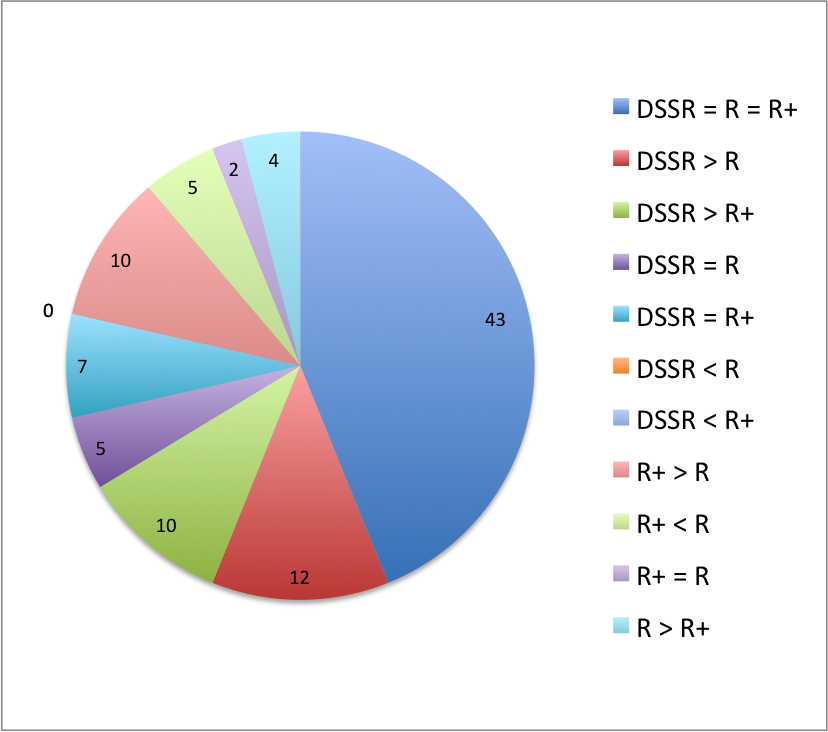
\includegraphics[width=8cm,height=7cm]{pie5.png}
%\caption{Division of result in to categories}
%\label{fig:pie}
%\end{figure}


%The first category contain 12 classes where DSSR strategy performs better than R. 
%The second category contain 10 classes where DSSR strategy performs better than R+. 
%The third category contain 5 classes where DSSR strategy and R performs equally well.
%The fourth category contain 7 classes where DSSR and R+ performs equally well. 
%The fifth category contain 10 classes where R+ performs better than R.
%The sixth category contain 5 classes where R performs better than R+.
%The seventh category contain 2 classes where R and R+ performs equally well.
%The eighth category contain 4 classes where R performs better than R+.
%Category 9 and 10 shows that neither R nor R+ performed better than DSSR strategy.
%The last category shows each strategy performing equally well for 43 classes. Expressing in percentage, 72\% classes do not show different behaviours whereas in 28\% of classes, the DSSR strategy performs better than R and R+ strategy. It is interesting to note that in no single case R and R+ strategies performed better than DSSR strategy. This is attributed to the fact that DSSR strategy possess the qualities of R and R+ and has the additional advantage of spot sweeping.

\subsection{The best default strategy in R, R+ \& DSSR}

Analysis of the experimental data revealed that DSSR strategy had an edge over R and R+. This is due to the additional feature of spot sweeping in DSSR strategy. In spite of the better performance of DSSR as compared to R and R+ strategies, the present study does not provide ample evidence to pick it as the best default strategy. This is primarily due to the overhead induced by DSSR strategy, discussed in Section~\ref{sec:discussion3}. Further study might provide some conclusive findings. 




%%%%%%%%%%%%%%%%%    DISCUSSION   %%%%%%%%%%%%%%%%%%%%

\section{Discussion}\label{sec:discussion3}
In this section we discuss various factors affecting the results of DSSR, R and R+ strategies including time taken, test duration, number of tests, number of failures, identification of first failure, level of coverage and threats to validity.

\textbf{Time taken by the strategies to execute equal number of test cases:}
The DSSR strategy took slightly more time (up to 5\%) than both R and R+ strategies which might be due to the feature of maintaining sets of interesting values during the execution. 

\textbf{Effect of test duration and number of tests on the results:}
If testing is continued for a long duration and sufficiently large number of tests are executed, in that case all three strategies might find the same number of unique failures. However for the same number of test cases, DSSR performed significantly better than R and R+ strategies. Further experiments are desirable to determine the comparative performance of the three strategies with respect to test duration and number of tests.

\textbf{Effect of number of failures on the results:} 
The DSSR strategy performed better when the number of failures was higher in the code. The reason might be that in case of more failures, the failure domains are more connected thus DSSR strategy might work better.

\textbf{Effect of identification of first failure on the results:}
During the experiments, It was noticed that quick identification of first failure was highly desirable in achieving better results from DSSR strategy. This was due to the feature of DSS which added the failure finding and surrounding values to the list of interesting values. However, when identification of first failure was delayed, no values were added to the list of interesting values and the DSSR performed equivalent to R+ strategy. This indicated that better ways of populating failure-inducing values were needed for sufficient leverage to DSSR strategy. As an example, the following piece of code would be unlikely to fail under the current setting:

\begin{lstlisting}
public void test(float value){
 if(value == 34.4445)   {
 	10/0;
 }
}
\end{lstlisting}

In this case, we could add constant literals from the SUT to the list of interesting values in a dynamic fashion. These literals can be obtained from the constant pool in the class files of the SUT. In the example above the value 34.4445 and its surrounding values would  be added to the list of interesting values before the test starts and the DSSR strategy would find the failure right away.

\textbf{Level of coverage:} Random strategies typically achieve low level of coverage~\cite{oriol2010yeti} and DSSR might be no exception. However it might be interesting to compare DSSR with R and R+ with respect to the achieved coverage.

\textbf{Threats to validity:} As usual with empirical studies, the present work might also suffer from a non-representative selection of classes. However selection in the study was made through random process and objective criteria to make it more representative.



%%%%%%%%%%%%%%%%%    RW   %%%%%%%%%%%%%%%%%%%%

\section{Related Work}\label{sec:rw}

Random testing is a popular technique with simple algorithm but proven to find subtle faults in complex programs and Java libraries~\cite{csallner2004jcrasher, pacheco2005eclat,claessen2011quickcheck}. Its simplicity, ease of implementation and efficiency in generating test cases make it the best choice for test automation~\cite{hamlet1994random}. Some of the well known automated tools based on R strategy includes JCrasher~\cite{csallner2004jcrasher}, Eclat~\cite{pacheco2005eclat}, AutoTest~\cite{ciupa2007experimental, ciupa2008artoo}, Jartege~\cite{oriat2005jartege} and YETI~\cite{oriol2010yeti, oriol2012random}.

In pursuit of better test results and lower overhead, many variations of R strategy have been proposed~\cite{chen2004mirror, chen2007quasi, chen2010adaptive, chan2006restricted, chen2004adaptive}. Adaptive random testing (ART), Quasi-random testing (QRT) and Restricted Random testing (RRT) achieved better results by selecting test inputs randomly but evenly spread across the input domain. ART through dynamic partitioning and MART are the two strategies developed to improve the performance of ART by reducing the overhead. This was achieved mainly by the even spread of test input to increase the chance of exploring the failure domains present in the input domain.

A more recent research study~\cite{yoo2012test} stresses on the effectiveness of data regeneration in close vicinity of the existing test data. Their findings showed up to two orders of magnitude more efficient test data generation than the existing techniques. Two major limitations of their study are the requirement of existing test cases to regenerate new test cases, and increased overhead due to ``meta heuristics search'' based on hill climbing algorithm to regenerate new data. In DSSR no pre-existing test cases are required because it utilises the border values from R+ and regenerate the data very cheaply in a dynamic fashion different for each class under test without any prior test data and with comparatively lower overhead. 
  
The R+ strategy is an extension of the R strategy in which interesting values, beside pure random values, are added to the list of test inputs~\cite{leitner2007reconciling}. These interesting values include border values which have high tendency of finding failures in the given SUT~\cite{beizer2003software}. Results obtained with R+ strategy showed significant improvement over R strategy~\cite{leitner2007reconciling}. DSSR strategy is an extension of R+ strategy which starts testing as R+ until a failure is found and then switches to dirt spot sweeping.

%It is interesting that numerous efforts have been made to discover the fault domains~\cite{Chen2010, Chen2005, Chan2002, Chen2004a, Chen2003}, etc. but in our knowledge, none has been published on covering/sweeping all the faults lying in a specific domain once it has been discovered.


A common practice to evaluate performance of an extended strategy is to compare the results obtained by applying the new and existing strategy to identical programs~\cite{hamlet1990partition, duran1984evaluation, gutjahr1999partition}. Arcuri et al.~\cite{arcuri2012random}, stress on the use of random testing as a baseline for comparison with other test strategies. We followed the procedure and evaluated DSSR strategy against R and R+ strategies under identical conditions.

In our experiments we selected projects from the Qualitas Corpus~\cite{tempero2010qualitas} which is a collection of open source java programs maintained for independent empirical research. The projects in Qualitas Corpus are carefully selected that spans across the whole set of java applications~\cite{oriol2012random, tempero2010empirical, tempero2008empirical}.


%%%%%%%%%%%%%%%%%    CONCLUSIONS   %%%%%%%%%%%%%%%%%%%%


\section{Summary}\label{sec:conc}
The main goal of the present study was to develop a new random strategy which could find more failures in a lower number of test cases. We developed the ``DSSR strategy'' as an extension of R+, based on the assumption that in a significant number of classes, failure domains are contiguous. The DSS feature of DSSR strategy adds neighbouring values of the failure finding value to the list of interesting values. The strategy was implemented in the random testing tool YETI to test 60 classes from Qualitas Corpus, 30 times each with each of the three strategies i.e. R, R+ and DSSR. The newly developed DSSR strategy uncovered more unique failures than both R and R+ strategies with a 5\% overhead. We found out that for 7 (12\%) classes DSSR was significantly better than both R+ and R, for 8 (13\%) classes DSSR performed significantly better than R, while in 2 (3\%) classes DSSR performed significantly better than R+. In all other cases, performance of DSSR, R and R+ showed no significant difference. On overall basis, DSSR produced encouraging results. 

\begin{figure}[h]
\centering
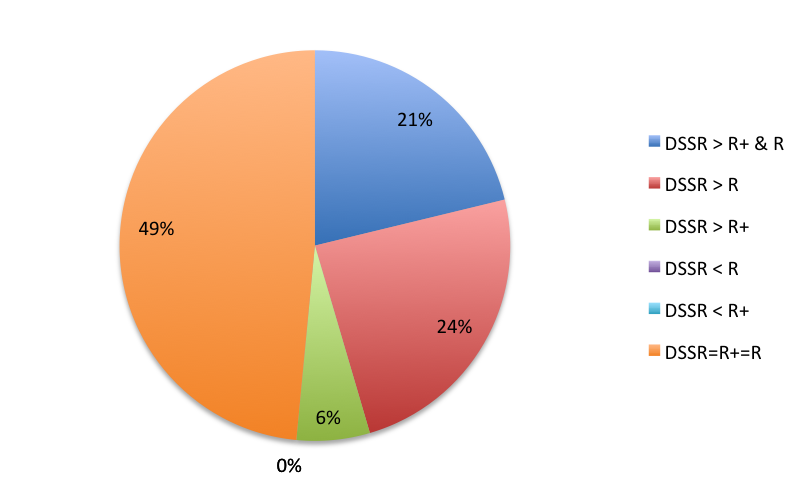
\includegraphics[width=14cm,height=9cm]{chapter4/resultsOfDSSRPie.png}
\caption{Results of DSSR strategy in comparison to Random and Random+}
\label{fig:resultsOfDSSRPie}
\end{figure}



